\documentclass[12pt]{article}
\usepackage[a4paper, top=2.5cm, bottom=2.5cm, left=1.5cm, right=1.5cm]{geometry}
\usepackage{amsmath, amsfonts, amssymb, mathtools}
\usepackage{fancyhdr, setspace, parskip}
\usepackage{graphicx, caption, subfig, array, multirow}
\usepackage{hyperref, enumitem, cancel}
\usepackage[T1]{fontenc}
\usepackage{tgtermes}
\usepackage[dvipsnames]{xcolor}
\usepackage[subfigure]{tocloft}
\usepackage{titlesec}
\usepackage{lipsum}  
\usepackage{tcolorbox}
\usepackage{float}
\usepackage{listings}
\tcbuselibrary{xparse}

\colorlet{codecolor}{black!30}
\newcommand{\codebox}[1]{%
  \colorbox{codecolor}{\ttfamily \detokenize{#1}}%
}

\definecolor{DarkBlue}{RGB}{10, 0, 80}
\definecolor{codegreen}{rgb}{0,0.6,0}
\definecolor{codegray}{rgb}{0.5,0.5,0.5}
\definecolor{codepurple}{rgb}{0.58,0,0.82}
\definecolor{backcolour}{rgb}{0.95,0.95,0.92}

\lstdefinestyle{mystyle}{
    backgroundcolor=\color{backcolour},   
    commentstyle=\color{codegreen},
    keywordstyle=\color{magenta},
    numberstyle=\tiny\color{codegray},
    stringstyle=\color{codepurple},
    basicstyle=\ttfamily\footnotesize,
    breakatwhitespace=false,         
    breaklines=true,                 
    captionpos=b,                    
    keepspaces=true,                 
    numbers=left,                    
    numbersep=5pt,                  
    showspaces=false,                
    showstringspaces=false,
    showtabs=false,                  
    tabsize=2
}

\lstset{style=mystyle}
% Hyperlink setup
\hypersetup{
    colorlinks=true,
    linkcolor=DarkBlue,
    filecolor=BrickRed,      
    urlcolor=RoyalBlue,
}

% Header and footer customization
\fancyhead{}
\fancyhead[L]{
{\fontfamily{lmss}{\color{DarkBlue}
\textbf{\leftmark}
}}
}
\fancyhead[R]{
{\fontfamily{ppl}\selectfont {\color{DarkBlue}
{Deep RL [Spring 2025]}
}}
}

\fancyfoot{}
\fancyfoot[C]{
{\fontfamily{lmss}{\color{BrickRed}
\textbf{\thepage}
}}
}

\renewcommand{\sectionmark}[1]{ \markboth{\thesection\quad #1}{} }

\renewcommand{\headrule}{{\color{BrickRed}\hrule width\headwidth height 0.5pt}}
\renewcommand{\footrulewidth}{0pt}


% Table of Contents customizations
\renewcommand{\cftsecafterpnum}{\vskip6pt}
\renewcommand{\cftsubsecafterpnum}{\vskip3pt}
\renewcommand{\cftsubsubsecafterpnum}{\vskip3pt}
\renewcommand{\cftsecfont}{\sffamily\large}
\renewcommand{\cftsubsecfont}{\sffamily}
\renewcommand{\cftsubsubsecfont}{\sffamily}
% \renewcommand{\cftsecdotsep}{1}
\renewcommand{\cftsubsecdotsep}{1}
\renewcommand{\cftsubsubsecdotsep}{1}


% Section title styles
\titleformat*{\section}{\LARGE\bfseries\color{DarkBlue}}
\titleformat*{\subsection}{\Large\bfseries\color{DarkBlue}}
\titleformat*{\subsubsection}{\large\bfseries\color{DarkBlue}}

\definecolor{light-gray}{gray}{0.95}
\newcommand{\code}[1]{\colorbox{light-gray}{\texttt{#1}}}

% Start of the document
\pagestyle{fancy}

%%%%%%%%%%%%%%%%%%%%%%%%%%%%%%%%%%%%%%%%%%%%%%%%%

\begin{document}

\pagenumbering{gobble}
\thispagestyle{plain}

\begin{center}

\vspace*{-1.5cm}
\begin{figure}[!h]
    \centering
    
\includegraphics[width=0.7\linewidth]{figs/cover-std.png}
\end{figure}

{
\fontfamily{ppl}

{\color{DarkBlue} {\fontsize{30}{50} \textbf{
Deep Reinforcement Learning
}}}

{\color{DarkBlue} {\Large
Professor Mohammad Hossein Rohban
}}
}


\vspace{20pt}

{
\fontfamily{lmss}


{\color{RedOrange}
{\Large
Homework 1:
}\\
}
{\color{BrickRed}
\rule{12cm}{0.5pt}

{\Huge
Introduction to RL
}
\rule{12cm}{0.5pt}
}

\vspace{10pt}

{\color{RoyalPurple} { \small By:} } \\
\vspace{10pt}

{\color{Blue} { \LARGE Amir Kooshan Fattah Hesari } } \\
\vspace{5pt}
{\color{RoyalBlue} { \Large 401102191 } }


\vspace*{\fill}
\begin{center}
\begin{tabular}{cc}
    
\includegraphics[width=0.16\linewidth]{figs/sharif-logo.png} & 
\includegraphics[width=0.16\linewidth]{figs/riml-logo.png} \\
\end{tabular}
\end{center}

\vspace*{-.25cm}

{\color{YellowOrange} {
\rule{8cm}{0.5pt} \\
\vspace{2pt}
\large Spring 2025}
}}
\vspace*{-1cm}

\end{center}

%%%%%%%%%%%%%%%%%%%%%%%%%%%%%%%%%%%%%%%%%%%%%%%%%

\newpage
\pagenumbering{gobble}
\thispagestyle{plain}
{\fontfamily{lmss}\selectfont {\color{BrickRed} \textbf{\tableofcontents} }}

{\fontfamily{lmss}\selectfont {\color{DarkBlue}

\subsection*{Grading}

The grading will be based on the following criteria, with a total of 100 points:

\[
\begin{array}{|l|l|}
\hline
\textbf{Task} & \textbf{Points} \\
\hline
\text{Task 1: Solving Predefined Environments} & 45 \\
\text{Task 2: Creating Custom Environments} & 45 \\

\hline
\text{Clarity and Quality of Code} & 5 \\
\text{Clarity and Quality of Report} & 5 \\
\hline
\text{Bonus 1: Writing a wrapper for a known env} & 10 \\
\text{Bonus 2: Implementing pygame env } & 20 \\
\text{Bonus 3: Writing your report in Latex } & 10 \\
\hline
\end{array}
\]

\textbf{Notes:}
\begin{itemize}
    \item Include well-commented code and relevant plots in your notebook.
    \item Clearly present all comparisons and analyses in your report.
    \item Ensure reproducibility by specifying all dependencies and configurations.
\end{itemize}

}

%%%%%%%%%%%%%%%%%%%%%%%%%%%%%%%%%%%%%%%%%%%%%%%%%

\newpage
\pagenumbering{arabic}

{\fontfamily{lmss}\selectfont {\color{DarkBlue}

\section{Task 1: Solving Predefined Environments [45-points]}
\textcolor{red}{\textbf{Important Note :} Due to the large size, the chart in the notebook file have been commented out, and their images have been included in the report. If they were note commented , the final size of the notebook would be 100 Mb. The TAs can uncomment and check the correctness of the plots.}
\subsection{Learning curves}
From the given environments, I chose the \textbf{Taxi} and \textbf{Cartpole} environment. First by using the gymnaisum pre-wrapped function \codebox{gymnasium.make() } i loaded the Cartpole environment to \codebox{env1}. It's action space has 2 values indicating the direction of the fixed force the cart is pushed with.
\begin{itemize}
 \item 0 : Push cart to the left
 \item 1 : Push cart to the right
\end{itemize}
It's observation space (state space) is a \codebox{ndarray} with dimensions \codebox{(4,)}.\\
Then by loading the \codebox{PPO,A2C,DQN} algorithms from the \codebox{stable_baselines3} library , I traind three different models with these algorithms and saved the amount of reward in each episode by using the \codebox{tensorboard_log} option of the algorithm's functions. After training each model I used the \codebox{del model} to free up some storage and memory.
The learning curves are as follows :
\begin{figure}[H]
    \centering
    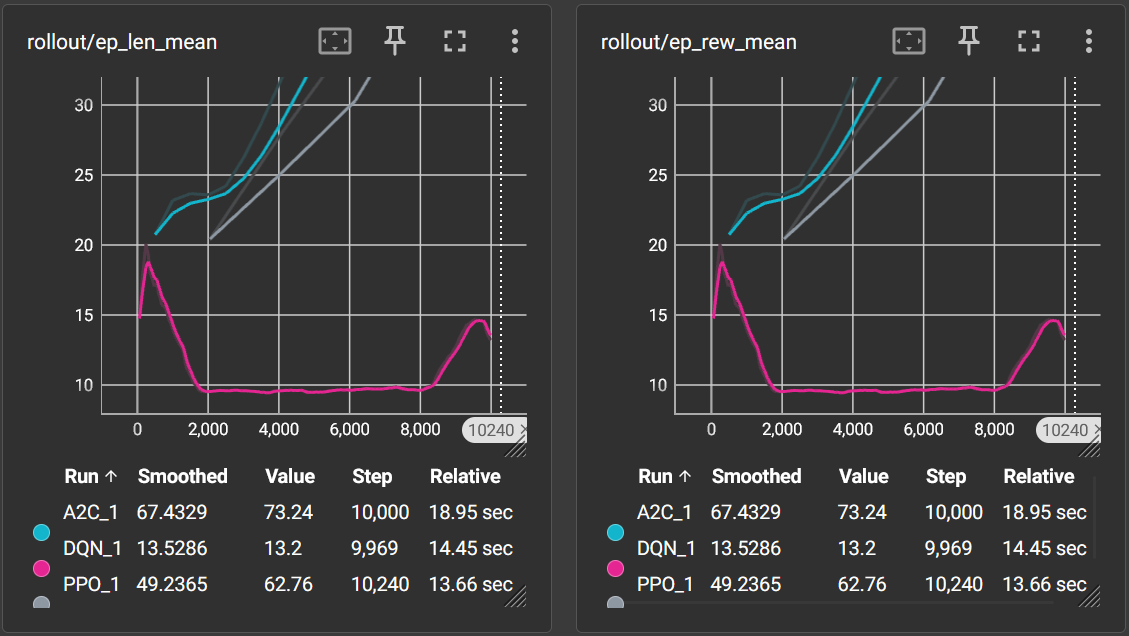
\includegraphics[width = 0.85\textwidth]{figs/learning_curve_normal.png}
    \caption{Learning curve of three different algorithms : PPO , A2C, and DQN for the CartPole-v1 environment }
\end{figure}
\begin{figure}[H]
    \centering
    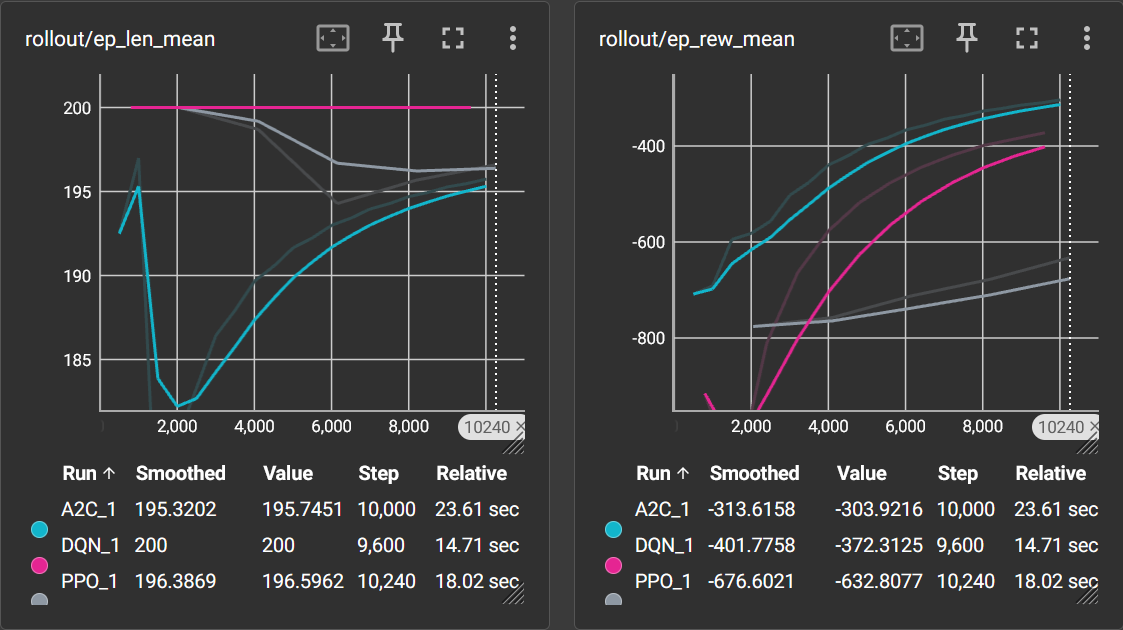
\includegraphics[width = 0.85\textwidth]{figs/learning_curve_taxi_noraml.png}
    \caption{Learning curve of three different algorithms : PPO , A2C, and DQN for the Taxi-v3 environment }
\end{figure}
We see that the reward in the \textbf{A2C} algorithm is better than the other two. By playing with the number of episodes we would also get the same results.\\
\subsection{Playing with hyperparameters} we play with the hyperparameters and try to see how this will change the performance of the models. For the PPO algorithm we examin these hyperparameters :
\begin{itemize}
 \item learning-rate: 4e-4, n-steps: 1536, batch-size: 96, gamma: 0.985, clip-range: 0.25
 \item learning-rate: 8e-4,n-steps: 768, batch-size: 48, gamma: 0.96, clip-range: 0.25
 \item learning-rate: 6e-4,n-steps: 3584, batch-size: 160,gamma: 0.94, clip-range: 0.15 
\end{itemize}
and for the DQN algorithm we examin these hyperparameters :
\begin{itemize}
 \item learning-rate: 1e-3, gradient-steps: 1, batch-size: 64, gamma: 0.99, tau: 1.0
 \item learning-rate: 5e-4, gradient-steps: 4, batch-size: 32, gamma: 0.95, tau: 0.01
 \item learning-rate: 2e-4, gradient-steps: 8, batch-size: 128, gamma: 0.97, tau: 0.05 
\end{itemize}
For the second environment we change the hyperparameters just a little bit as follows , for PPO : 
\begin{itemize}
 \item learning-rate: 3e-4, n-steps: 1436, batch-size: 86, gamma: 0.995, clip-range: 0.25
 \item learning-rate: 7e-4,n-steps: 568, batch-size: 38, gamma: 0.92, clip-range: 0.35
 \item learning-rate: 5e-4,n-steps: 2584, batch-size: 140,gamma: 0.91, clip-range: 0.15 
\end{itemize}
and for DQN :
\begin{itemize}
 \item learning-rate: 2e-3, gradient-steps: 1, batch-size: 64, gamma: 0.99, tau: 1.0
 \item learning-rate: 8e-4, gradient-steps: 3, batch-size: 32, gamma: 0.95, tau: 0.01
 \item learning-rate: 5e-4, gradient-steps: 6, batch-size: 128, gamma: 0.97, tau: 0.05 
\end{itemize}
\begin{figure}[H]
    \centering
    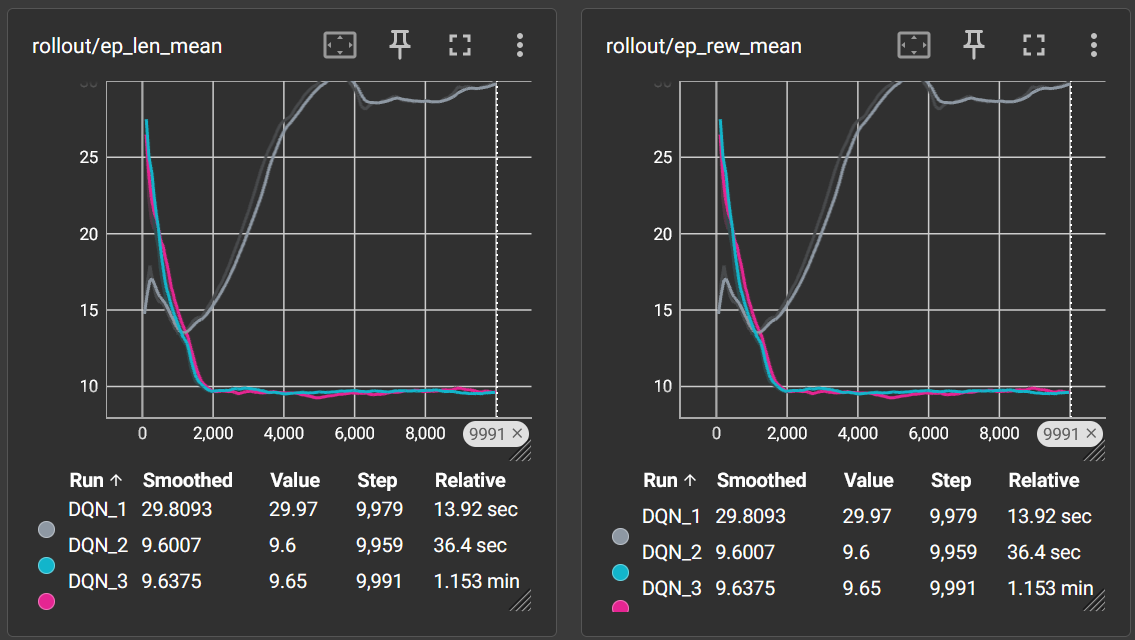
\includegraphics[width = 0.75\textwidth]{figs/dqn_cartpole_hyper.png}
    \caption{Learning curve of three different sets of hyperparameters for DQN algorithm for the CartPole-v1 environment}
\end{figure}
\begin{figure}[H]
    \centering
    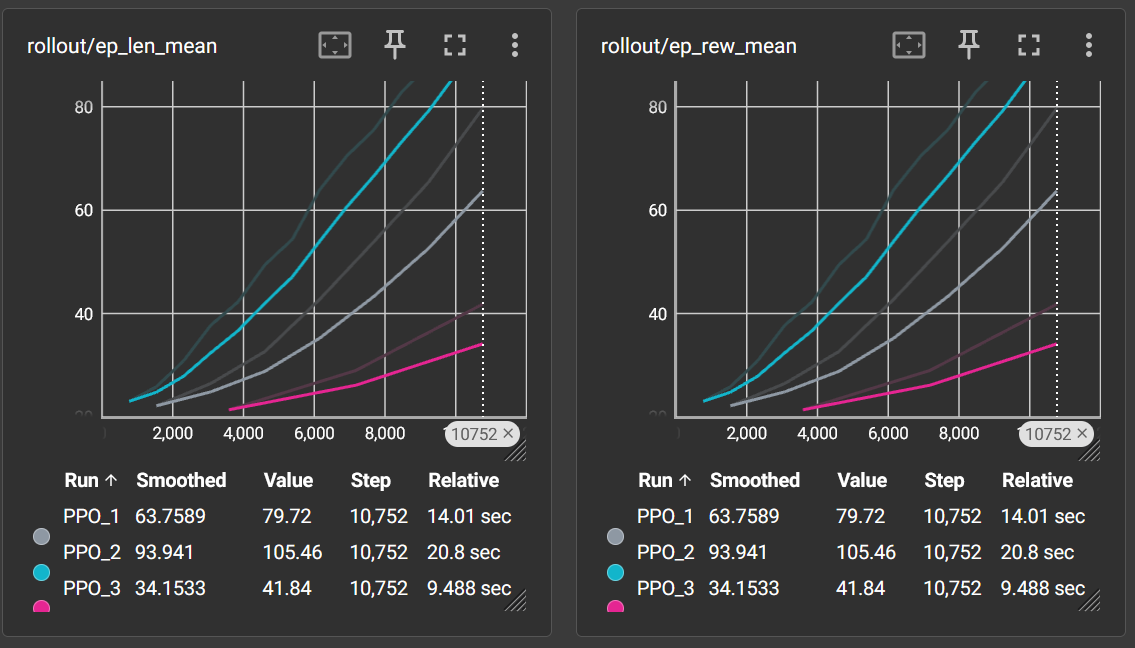
\includegraphics[width = 0.75\textwidth]{figs/ppo_cartpole_hyper.png}
    \caption{Learning curve of three different sets of hyperparameters for PPO algorithm for the CartPole-v1 environment}
\end{figure}
\begin{figure}[H]
    \centering
    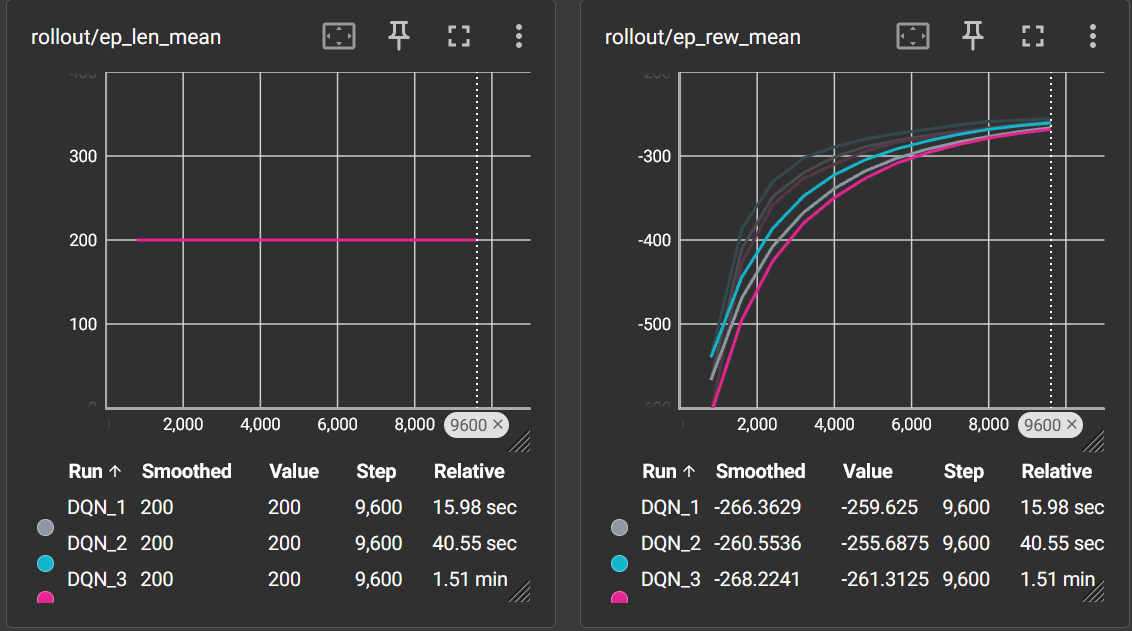
\includegraphics[width = 0.75\textwidth]{figs/taxi_dqn_hyperparameters.png}
    \caption{Learning curve of three different sets of hyperparameters for DQN algorithm for the Taxi-v3 environment}
\end{figure}
\begin{figure}[H]
    \centering
    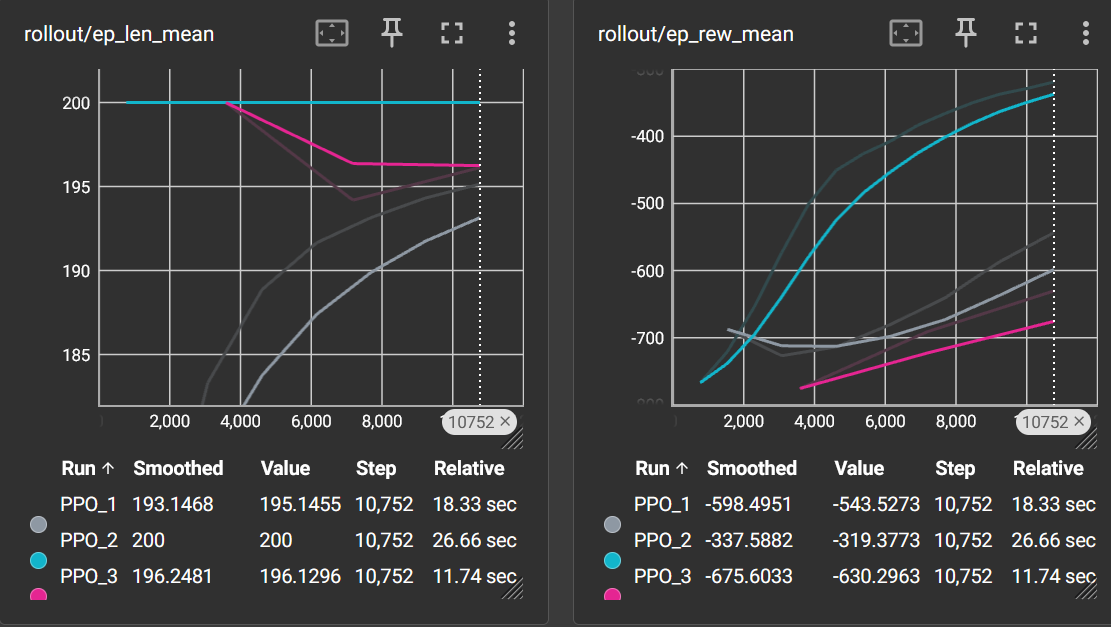
\includegraphics[width = 0.75\textwidth]{figs/taxi_ppo_hyperparameters.png}
    \caption{Learning curve of three different sets of hyperparameters for PPO algorithm for the Taxi-v3 environment}
\end{figure}
\subsection{Reward Function Wrapper (Bonus)} I wrote the following wrapper for reward function :
\begin{lstlisting}[language=Python, caption=Reward Wrapper]
from gymnasium import RewardWrapper
class RewardFormula(RewardWrapper):
  def reward(self, reward):
        return reward * 2 + 1
EnvWrapped = make_vec_env(lambda: RewardFormula(gym.make("CartPole-v1", render_mode="rgb_array")), n_envs=1) 
\end{lstlisting}
The use of \codebox{lambda} is due to the fact that the \codebox{RewardFormula} class expects an instance of the type \codebox{env} , not \codebox{VecEnv}, therefore we use this function to pass it to \codebox{make_vec_env} function.
\begin{figure}[H]
    \centering
    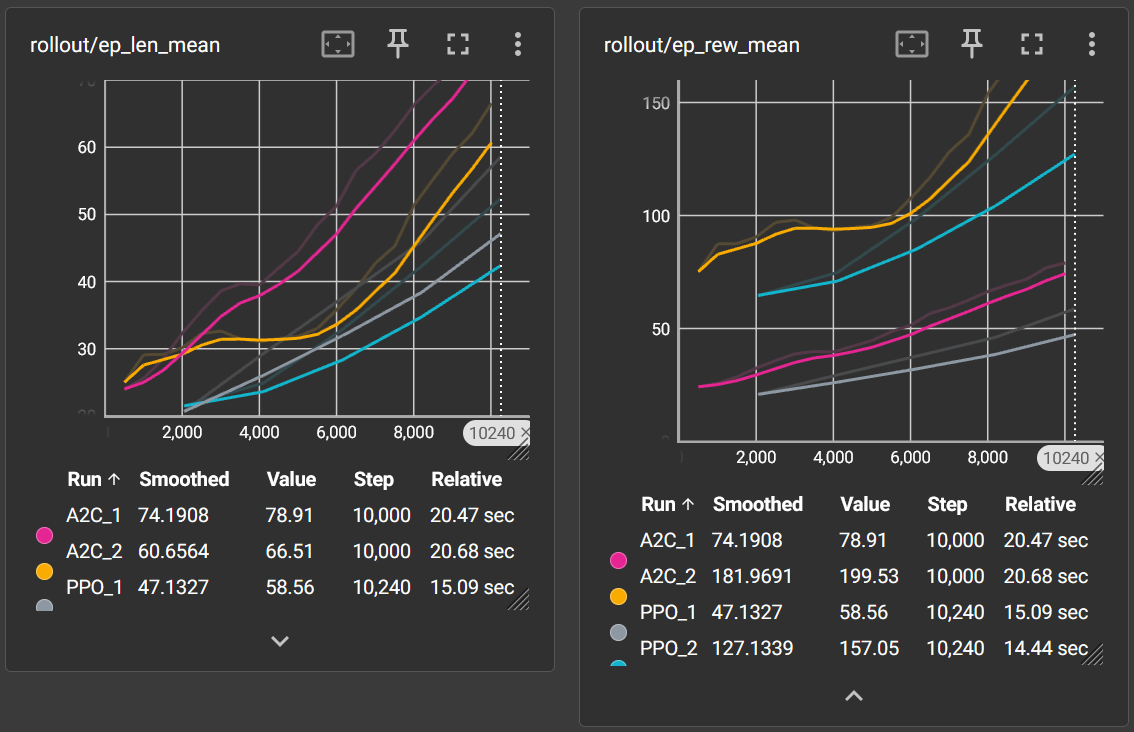
\includegraphics[width = 0.75\textwidth]{figs/reward_wrapper.png}
    \caption{Learning curve of the main PPO and A2C algorithms and their repsective wrapped one for the CartPole-v1 environment}
\end{figure}
\begin{figure}[H]
    \centering
    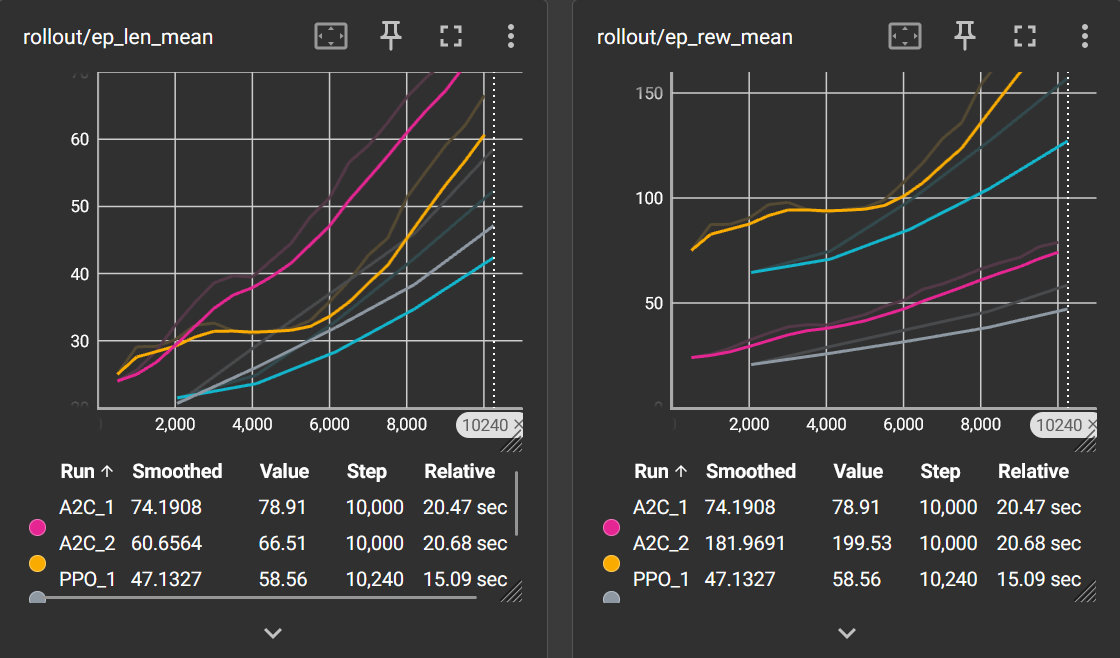
\includegraphics[width = 0.75\textwidth]{figs/taxi_reward_wrapped.png}
    \caption{Learning curve of the main PPO and A2C algorithms and their repsective wrapped one for the Taxi-v3 environment}
\end{figure}
We see that wrapping the reward function and returning \codebox{reward * 2 + 1} is evident in the plots that it makes the reward greater for both of the algorithms.\\
\subsection{SL fitness discussion (Bonus)}
In well-defined environments like CartPole and Taxi, SL can work well if you have a high-quality set of expert demonstrations and it can be an be very sample-efficient compared to RL, which learns through trial and error.\\
On the other hand some problems might rise. SL learns from a fixed dataset of expert demonstrations. When the learned policy makes a mistake, it may visit states that are not well-represented in the training data and distribution mismatch (covariate shift) leads to compounding errors and degrades the performance.\\
Another common problem is that if in the settings of the problem the reward is sparse or we have a long horizon , small deviations from expert behavior can lead the agent far from the rewarding states where SL might fail to provide the necessary corrections for these deviations, whereas RL methods�through iterative trial and error�can learn to navigate these long-horizon challenges.
}}
%%%%%%%%%%%%%%%%%%%%%%%%%%%%%%%%%%%%%%%%%%%%%%%%%

\newpage

{\fontfamily{lmss}\selectfont {\color{DarkBlue}

\section{Task 2: Creating Custom Environments [45-points]}
\subsection{Discussion on implementation and modification}
Based on the given tasks, first we implement a new \codebox{class} name \textbf{YourAwesomeEnvironment} which is a subclass of the \codebox{gym.Env} class.
In the \codebox{__init__} method, we declare the basics of an environment; the position of tha agent , the position of the target , place of obstacles on the grid, the action space, and the observation space.\\
The action space contains the actions that the agent can do which are four ; going \textbf{up , down , right, and left}.\\
The observation space contains all the possible positions of the agent and target on the grid.
In the \codebox{step(self,action)} function we define what happens to the position of the agent if a certain action is taken, e.g. if \codebox{action == 1} then the horizontal position of the agent increases by amount of one. If the new position is on an obstacle the position isn't updated and another action is taken.\\
Then if the agent's position and that of target's become the same, meaning they are at the same place, the agent is rewarded a value of 10 and the episode is over.\\
The \codebox{rest} function return the agent to its original place and sets everything else to default.
Since we will need to compute observations both in \codebox {Env.reset()} and \codebox {Env.step()}, it is often convenient to have a method \codebox {_get_obs} that translates the environment�s state into an observation.
The \codebox{render} function was implemented using \textbf{ChatGPT} because I didn't know what to render or even how to render using the \codebox{env.render} option, \codebox{it's extra} and for this simple environment we didn't have any need for a close method.\\
\textbf{Also} changing the hyperparameters in the used algorithms may lead to better and faster learning or chaning the reward given at different states.
\subsection{Training results, learning curves, and observations}
For trainig results using the PPO algorithm we have the following output :
\begin{figure}[htp]

\centering
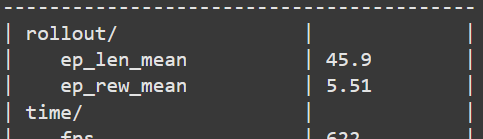
\includegraphics[width=.3\textwidth]{figs/reward_custom_1.png}\hfill
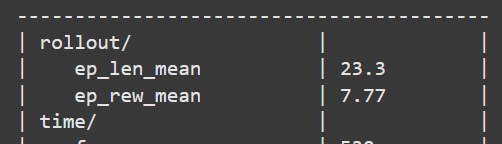
\includegraphics[width=.3\textwidth]{figs/reward_custom_2.png}\hfill
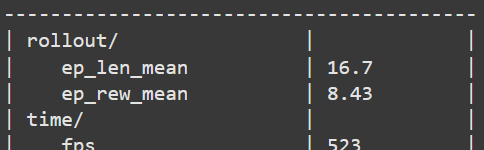
\includegraphics[width=.3\textwidth]{figs/reward_custom_3.png}
\caption{The training results of the custom environment on the PPO algorithm}
\end{figure}
As it is clear in the pictures , the average reward return per episode is increasing which means that the training is going well.
Also comparing the PPO and the DQN algorithm yields the following results :
\begin{figure}[H]
    \centering
    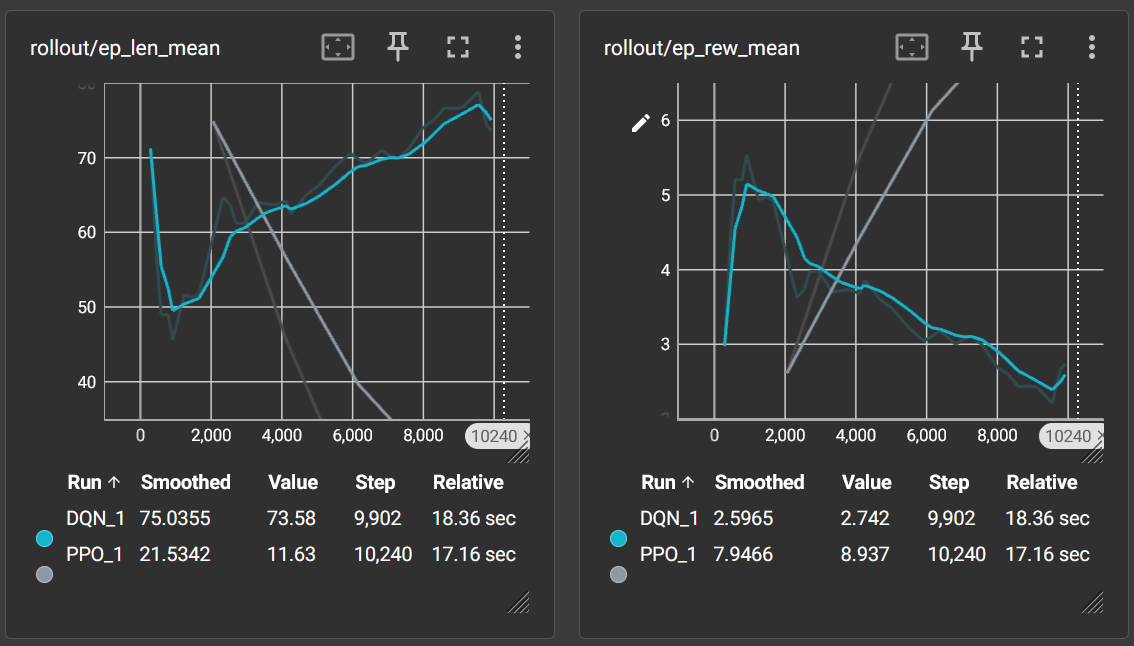
\includegraphics[width = 0.75\textwidth]{figs/custom_reward_dqn_ppo.png}
    \caption{Learning curves of the PPO and DQN algorithms in the custom environment}
\end{figure}
Also changing the hyperparameters and comparing the results with each other is as follows:
\begin{figure}[htp]

\centering
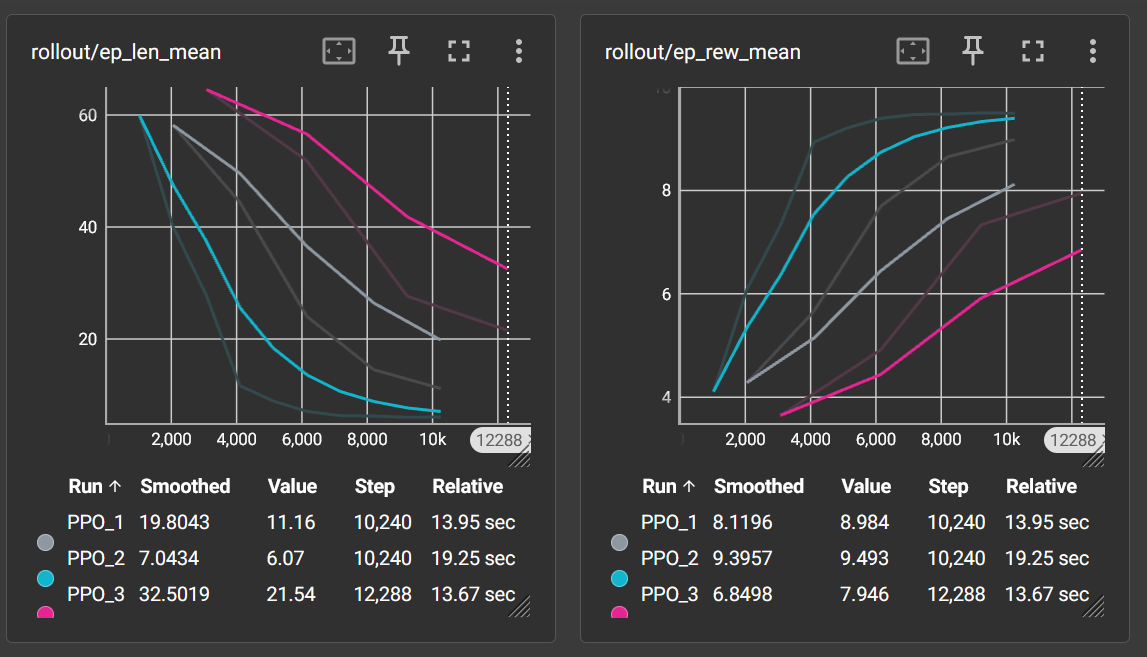
\includegraphics[width=.45\textwidth]{figs/ppo_custom_hyper.png}\hfill
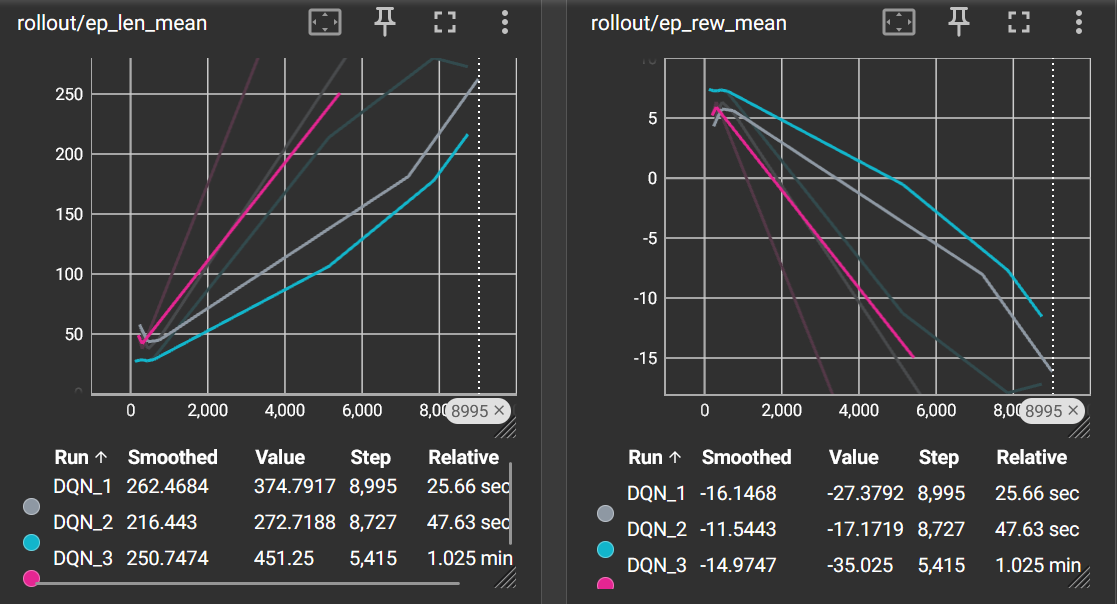
\includegraphics[width=.45\textwidth]{figs/dqn_custom_hyper.png}
\caption{The training results of the custom environment on the PPO algorithm}
\end{figure}
\subsection{Code of the environment}
The main components of the custom environment are:
\begin{lstlisting}[language=Python, caption=Initialization]
class YourAwesomeEnvironment(gym.Env):
    def __init__(self, size=4, obstacles):
        super().__init__()
        self.size = size
        self.agent_pos = [0, 0]
        self.target_pos = [size - 1, size - 1] 
        obstacles = [(1, 1), (2, 2)]
        self.obstacles = set(obstacles)
        self.action_space = spaces.Discrete(4)
        self.observation_space = spaces.Dict({
            "agent": spaces.MultiDiscrete([size, size]),
            "target": spaces.MultiDiscrete([size, size]),
        })
\end{lstlisting}
\begin{lstlisting}[language=Python, caption=step method]
    def step(self, action):
        x, y = self.agent_pos
        # Compute new position
        new_x, new_y = x, y
        if action == 0 and y > 0:   # Move Left
            new_y -= 1
        elif action == 1 and y < self.size - 1:  # Move Right
            new_y += 1
        elif action == 2 and x > 0:   # Move Up
            new_x -= 1
        elif action == 3 and x < self.size - 1:  # Move Down
            new_x += 1
        if (0 <= new_x < self.size and 0 <= new_y < self.size) and (new_x, new_y) not in self.obstacles:
            self.agent_pos = [new_x, new_y]  # Update position if it's a valid move
        reward = -0.1  # Small penalty per step
        done = False
        if self.agent_pos == self.target_pos:
            reward = 10  # Large reward for reaching the goal
            done = True  # Episode ends
        return self._get_obs(), reward, done, False, {}
\end{lstlisting}
\begin{lstlisting}[language=Python, caption=reset method]
    def reset(self, seed=None, options=None):
        self.agent_pos = [0, 0]
        return self._get_obs(), {}
\end{lstlisting}
A complete explanation of different parts is given in subsection 2.1.
}}
%%%%%%%%%%%%%%%%%%%%%%%%%%%%%%%%%%%%%%%%%%%%%%%%%


\newpage

{\fontfamily{lmss}\selectfont {\color{DarkBlue}

\section{Task 3: Pygame for RL environment [20-points]}
\subsection{Updated Pygame Environments}
In the given notebook there was no pre-existing environment for this part, so creating one from scratch required a little of digging and searching.
\begin{lstlisting}[language=Python, caption=Initialization method]
   def __init__(self, grid_size=10, cell_size=40, render_mode="human"):
        self.grid_size = grid_size      # Number of cells per dimension.
        self.cell_size = cell_size      # Pixel size of each cell.
        self.width = self.grid_size * self.cell_size
        self.height = self.grid_size * self.cell_size
        self.render_mode = render_mode
        self.action_space = spaces.Discrete(4)
        self.observation_space = spaces.Box(low=0, high=self.grid_size - 1, shape=(2,), dtype=np.int32)
        if self.render_mode == "human":
            pygame.init()
            self.screen = pygame.display.set_mode((self.width, self.height))
            pygame.display.set_caption("GridWorld Environment")
            self.clock = pygame.time.Clock()
        self.agent_color = (0, 255, 0)
        self.goal_color = (255, 0, 0)
        self.obstacle_color = (0, 0, 255)
        self.bg_color = (255, 255, 255)
        self.reset()
\end{lstlisting}
Just like the custom environment we create a subclass of the \codebox{gym.Env} class and initialize it in the same way, \textbf{except} that we specify a \codebox{render_mode} and initialize a pygame screen so that the game can be shown on it and give color to different components. Everything else like the agent position and obstacles and the size and spaces and ... are implemented in the same way as before.\\
The \codebox{step} and \codebox{reset} function explanations are like those given in Task 2.\\
\begin{lstlisting}[language=Python, caption=render method]
   def render(self):
        if self.render_mode is None:
            return
        self.screen.fill(self.bg_color)
        for x in range(0, self.width, self.cell_size):
            for y in range(0, self.height, self.cell_size):
                rect = pygame.Rect(x, y, self.cell_size, self.cell_size)
                pygame.draw.rect(self.screen, (200, 200, 200), rect, 1)
        for obs in self.obstacles:
            rect = pygame.Rect(obs[0] * self.cell_size, obs[1] * self.cell_size, self.cell_size, self.cell_size)
            pygame.draw.rect(self.screen, self.obstacle_color, rect)
        rect = pygame.Rect(self.goal_pos[0] * self.cell_size, self.goal_pos[1] * self.cell_size, self.cell_size, self.cell_size)
        pygame.draw.rect(self.screen, self.goal_color, rect)
        rect = pygame.Rect(self.agent_pos[0] * self.cell_size, self.agent_pos[1] * self.cell_size, self.cell_size, self.cell_size)
        pygame.draw.rect(self.screen, self.agent_color, rect)

        pygame.display.flip()
        self.clock.tick(30)
\end{lstlisting}
Given the state of the episode , it draws the rectangles, the agent, and the target given their updater locations in a 400 * 400 window. For defining the render function \textbf{ChatGPT} has been helpful.
\subsection{Screenshots of the modifications and explanations}
The explanations are given in the first part and changing the positions and the size of the grid and reward may cause different learning rates with different algorithms, but here we examin the PPO algorithm. The results are in the notebook and a screenshot of the created environment is as follows :
\begin{figure}[H]
    \centering
    \includegraphics[width = 0.85\textwidth]{figs/Pygame.png}
    \caption{Pygame environment}
\end{figure}
}}


%%%%%%%%%%%%%%%%%%%%%%%%%%%%%%%%%%%%%%%%%%%%%%%%%

\newpage

{\fontfamily{lmss}\selectfont {\color{DarkBlue}

\begin{thebibliography}{9}

\bibitem{SuttonBarto}
R. Sutton and A. Barto, \textit{Reinforcement Learning: An Introduction}, 2nd Edition, 2020. Available online: \url{http://incompleteideas.net/book/the-book-2nd.html}


\bibitem{StableBaselines3}
A. Raffin et al., "Stable Baselines3: Reliable Reinforcement Learning Implementations," GitHub Repository, 2020. Available: \url{https://github.com/DLR-RM/stable-baselines3}.

\bibitem{Gymnasium}
Gymnasium Documentation. Available: \url{https://gymnasium.farama.org/}.

\bibitem{Pygame}
Pygame Documentation. Available: \url{https://www.pygame.org/docs/}.

\bibitem{CS285}
CS 285: Deep Reinforcement Learning, UC Berkeley, Pieter Abbeel. Course material available: \url{http://rail.eecs.berkeley.edu/deeprlcourse/}.

\bibitem{Freepik}
\href{https://www.freepik.com/free-vector/cute-artificial-intelligence-robot-isometric-icon_16717130.htm}{Cover image designed by freepik}

\end{thebibliography}


}}

%%%%%%%%%%%%%%%%%%%%%%%%%%%%%%%%%%%%%%%%%%%%%%%%%

\end{document}
